%% This is an example first chapter.  You should put chapter/appendix that you
%% write into a separate file, and add a line \include{yourfilename} to
%% main.tex, where `yourfilename.tex' is the name of the chapter/appendix file.
%% You can process specific files by typing their names in at the 
%% \files=
%% prompt when you run the file main.tex through LaTeX.
\chapter{Partition Function Computation and Improvements}
\section{Introduction}

The partition function for a thermodynamic system of fixed volume, in
contact with a heat reservior with absolute temperature $T$, is
\begin{equation} Z = \sum_s e^{-E(s)/ RT }, \end{equation}
where $s$ denotes a particular state of the system, $E(s)$ is the
energy of that state, and $RT$ is the gas constant multiplied by the
temperature, specified above. Each particular term in the sum is
called that state's Boltzmann factor. The probability of a state is
then said to be its Boltzmann factor divided by the partition
function, or
\begin{equation} P(s) = \frac{1}{Z}e^{-E(s)/RT}.  \end{equation}
In our model an RNA strand is such a thermodynamic system, its
secondary structure is its state, and the rest of the cell is the
reservoir of heat. We assign each secondary structure an energy
according to the free energy model described in Chapter 1. According
to this model, the energy of a secondary structure is the sum of the
energies of its loops. 

To compute the partition function we must sum up every possible
secondary structure. There are many possible secondary structures, on
the order of $1.8^n$ where $n$ is the sequence length. However, the
computation of the partition function benefits greatly from the linear
nature of the energy model: it allows us to recursively define the
partition function. For example, say we have computed the full
partition function of a strand of $n$ bases, define a function $Q$
such that:
\begin{equation}
Q(i, j) = \text { sum of boltzmann factors for every structure contained between } i \text{ and } j.
\end{equation}
The full partition computation can therefore be represented as the
function $Q$ acting on the bounding two bases $1$ and $n$: 
\begin{equation}
 Q(1, n) = \sum_{s \text{ on } [1,n]} e^{-E(s)/RT}.
\end{equation}
If we now extend the strand by attaching a small hairpin to the end,
as pictured in Figure \ref{fig:attachedHairpin}, there is no need to
go back and recompute the energy of every single secondary structure,
rather we can just multiply the already-computed partition function by
the boltzmann factor of the hairpin turn (let $E(h)$ be the hairpin
energy) to get the new partition function:
\begin{figure}[h]
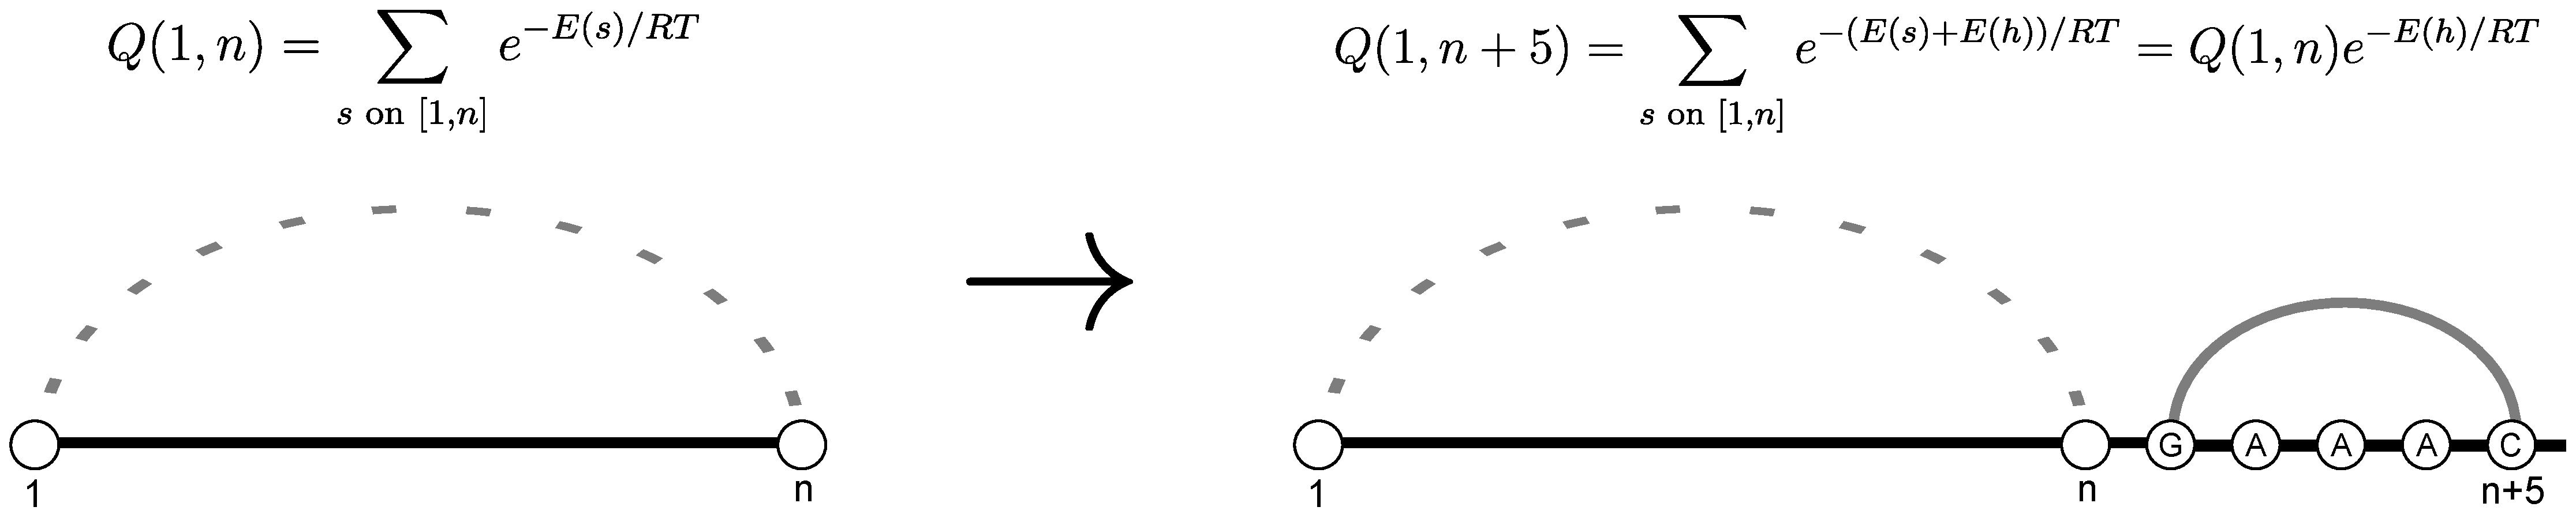
\includegraphics[width=\textwidth]{attachedHairpin.eps}
\caption{Extending the strand by adding an attached hairpin adds the
  energy of the hairpin to each structure. To compute the new
  partition function $Q(1, n+5)$, we do not need to sum the energies
  of all possible structures again, we can simply use the old value,
  $Q(1,n)$, and multiply it by the Boltzmann factor of the
  hairpin. This is the concept behind the dynamic programming
  algorithm.}
\label{fig:attachedHairpin}
\end{figure}
\begin{equation}
Q(1, n + 5) = \sum_{s \text{ on } [1,n]} e^{-(E(s) + E(h))/RT} = Q(1, n)e^{-E(h)/RT}. 
\end{equation}
This replaces an exponential-time computation (the sum), with a
constant time computation (multiplying the pre-computed $Q(1, n)$ with
the energy term). In general, this technique allows us to compute the
partition function efficiently, working up from $Q(1, 2)$ to
$Q(1,n)$. In computer science this technique is called dynamic
programming, a fancy name for the technique of storing the
results of a computation in a table for later use.

The dynamic programming algorithm for computing the partition function
of an RNA strands has several versions, depending on how in depth you
go with the energy model. The simplest algorithms allow for only
structures with nested base pairs. Nested means that the structure can
be represented with the parenthesis, for example
(((..((((....))))(((..)))..))), or without crossing pairs in expanded
loop diagrams such as the ones in Figure
\ref{fig:attachedHairpin}. Note that this kind of structure excludes
pseudoknots.  If you ignore psuedoknots, which is standard in the
field, and if you make an approximation that internal loops will never
exceed a certain length, the fastest algorithm runs in $O(n^3)$. We
believe that we can streamline this computation even more, taking
advantage of the fact that empirically, the number of probable base
pairs of a strand of length $n$ seems to grow like $n$, not
$n^2$. This is the same result we used to speed up the stochastic
traceback algorithm and potentially a partition function algorithm
that includes pseudoknots. The algorithm will be presented in its
simplest form, with more complicated versions available in the
appendices.

\section{Motivation}

There exists an efficient algorithm to find the minimum free energy
structure of a sequence. The fundamental algorithm for the MFE was
developed by Zuker and Steigler in 1981
\cite{zuker1981optimal}. However, perhaps counterintuitively, the MFE
structure is not always the structure that is found in nature, even
though natural systems tend to their lowest energy state. It is less
counterintuitive after seeing Figure \ref{fig:probMFE}. The
probability of any individual state is bounded from above by the MFE,
which approaches zero very quickly as the length of the sequence
increases.
\begin{figure}[t]
\centering
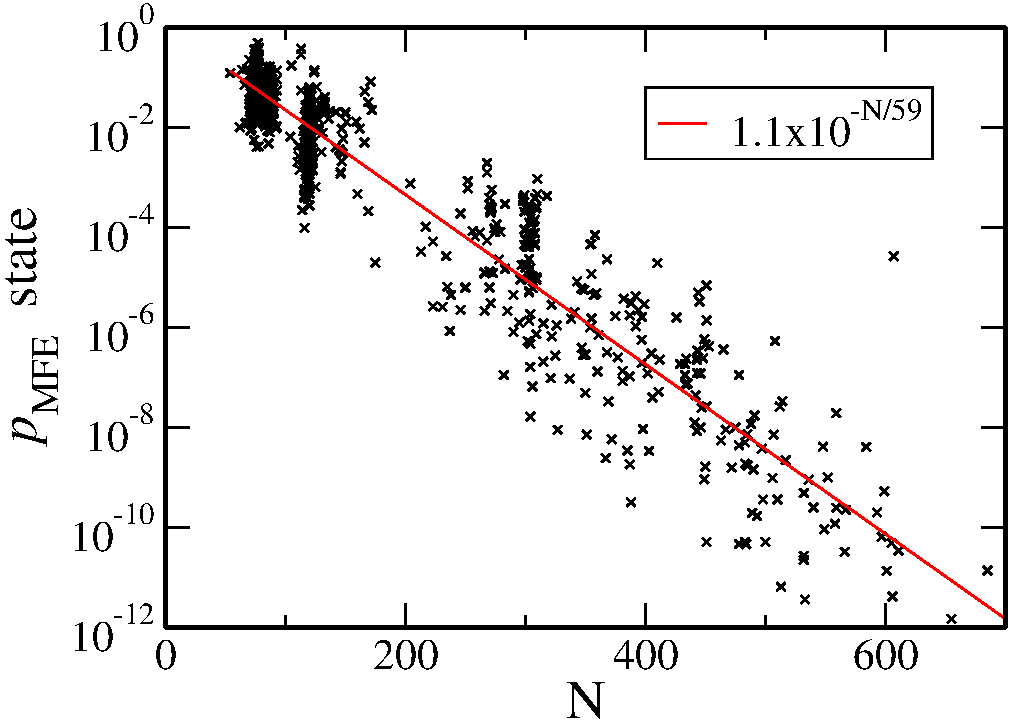
\includegraphics[width=.8\textwidth]{pMFE2.pdf}
\caption{A plot of probability of the MFE state as computed $P(MFE) =
  e^{-E_{min}/RT}/Z$ for sequences of many different lengths. For
  sequences of reasonable length, even though it is the most probable
  state, the MFE probability approaches floating point error. This
  forces us to approach probabilities differently, using sums of
  probabilities of many similar states instead of just one state. [TODO: where
    does this data come from?]}
\label{fig:probMFE}
\end{figure}
The encourages us to treat the probabilities of secondary structures
given to us by Boltzmann statistics as probability densities instead
of actual probabilities. The structure that is found in nature is most
likely going to be from the most probable macrostate, where we define
macrostate as following:
\begin{description}
\item[Macrostate:] A set of RNA secondary structures sufficiently
  close to a local energy minimum structure $s_{min}$. 
\end{description}
The ``sufficiently close'' in the definition is not widely agreed
upon, and has spawned several different techniques of defining and
computing RNA macrostates (see Clustering chapter).

This logic was presented by Ye Ding, Chi Yu Chan, and Charles
E. Lawrence in their 2005 paper ``RNA secondary structure prediction
by centroids in a Boltzmann weighted ensemble''
\cite{ding2005rna}. What they found that, as suspected, the MFE state
was not always a member of the most probable macrostate. Using a
method based on centroids of statistically sampled states, they found
that their method made 30\% fewer prediction errors, improving
positive predictive value by 46.5\% and sensitivity by 21.7\%. Figure
\ref{fig:centroidFig} is an illustration of this concept.
\begin{figure}[t]
\centering
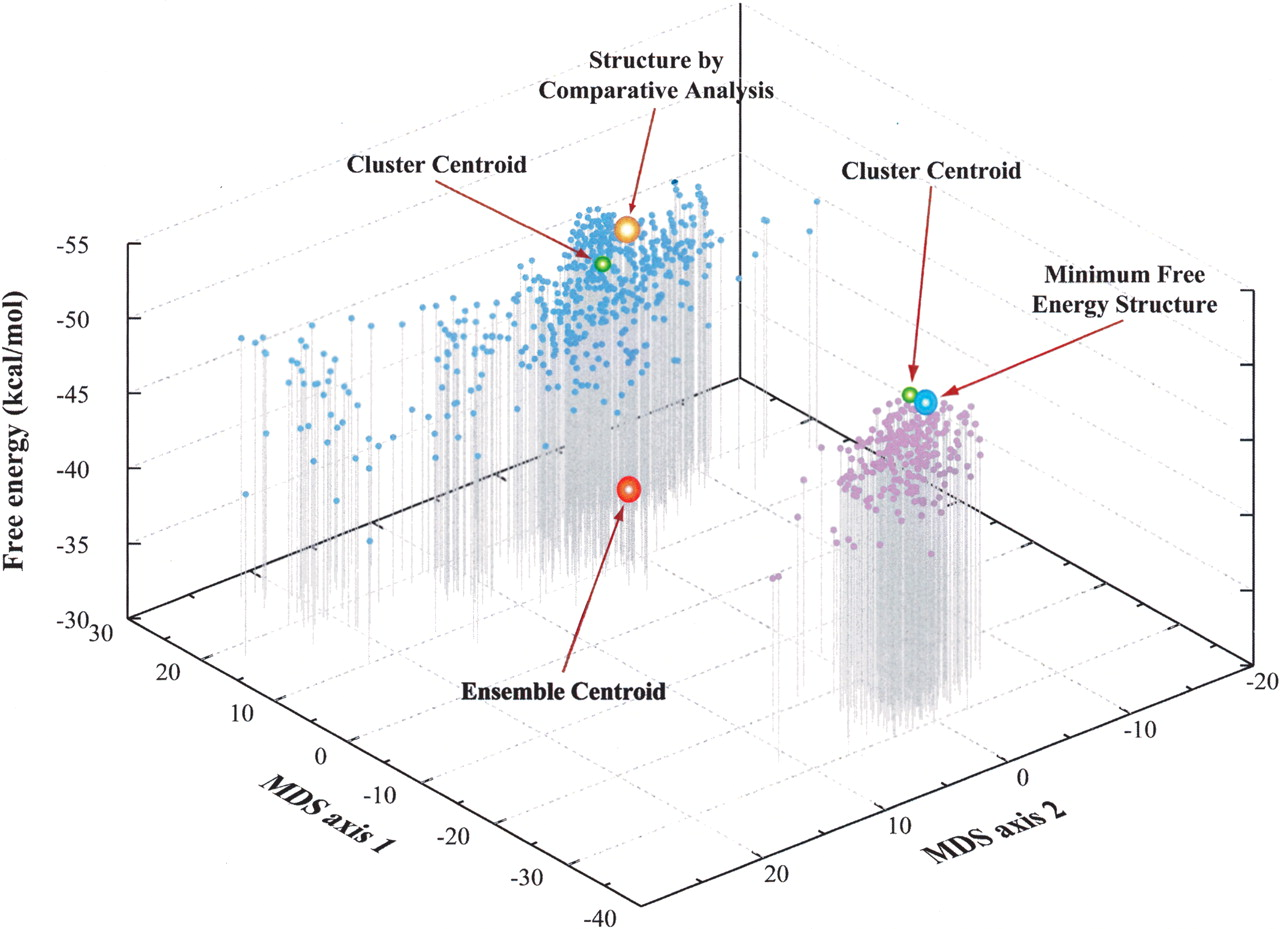
\includegraphics[width=.8\textwidth]{ensemble-centroid.jpg}
\caption{An RNA strand with mutliple macrostates, found by clustering
  analysis and plotted along 2 principle components. The MFE state is
  not in the most probably macrostate, neither is the ensemble
  centroid, but the macrostate centroid gives good predictions of
  secondary structure. Figure from Ding, Chu, \& Lawrence (2005).}
\label{fig:centroidFig}
\end{figure}

In all the clustering algoritms, since we must know boltzmann
statistics of different states, we must compute the partition
function. In certain situations, such as partition function
clustering, the partition function is recomputed several times. If the
partition function takes on the order of hours or days to compute,
this can make partition function clustering a major bottleneck in
whatever process RNA secondary structure prediction is being used
in. However in these situations it is also true that the partition
function is recomputed with almost the same conditions, just certain
pairs restricted. 

\begin{figure}[t]
\centering
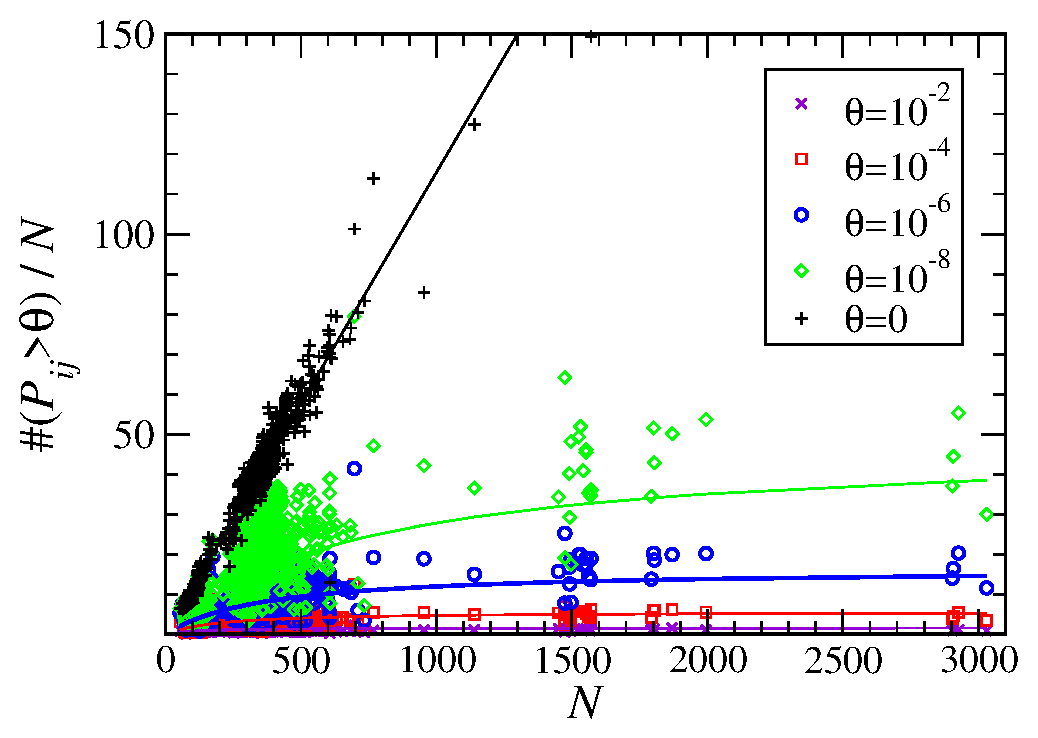
\includegraphics[width=.8\textwidth]{PijTheta5.eps} 
\caption{A plot of `number of pairs with probability greater than
  colored threshhold' vs length of sequence. If there is no threshold,
  the number of pairs possible goes up like $n^2$, but even with small
  thresholds such as requiring a pair to have probability greater than
  $10^{-8}$, the number of possible pairs goes flat as $n$
  increases. Therefore, a great amount of efficiency can be gained by
  restricting the pairs under consideration, while not sacrificing
  much accuracy since the thresholds are so low. }
\label{fig:probThresh}
\end{figure}

We've been able to show via experiment that the partition function
only admits roughly $O(n)$ pairs with probabilities above thresholds
around the machine precision limit. If we have the partition function
already computed, we can recompute it by only adding in pairs that
have sufficient probability. We can also extend this method: if a good
heuristic appears in the future, one that can eliminate a large number
of pairs, while being computationally cheap, we should be able to use
the results to speed up the partition function computation. This
motivates a method of computing the partition function using a
known-pairs heueristic to prune away unneccesary computation, and that
is what we have implemented.

\section{The Computation}

The standard way of computing the partition function involves filling
out a table where the $(i,j)$th member represents the partition
function for the substrand from base $i$ to base $j$,
$Q(i,j)$. Because the energy model for RNA is linear, $Q(i,j)$ can be
expressed as a function of nearby members of this table. This function
is called the recurrence relation for the partition function of
RNA. Because the free energy model is so complicated and has gone
through many iterations, differenct RNA folding software packages
implement different versions of the recurrence relation, and they vary
widely in complexity. This version is as simple as possible, there is
an energy penalty for starting a multiloop, $a$, and an energy penalty
for keeping a base unpaired, $b$, otherwise we hold to the standard
energy functions.

The definitive representation of the recurrence relation for RNA was
formulated in 1990 by J.S. McCaskill in his paper \emph{The
  Equilibrium Partition Function and Base Pair Binding Probabilities
  for RNA Secondary Structure} \cite{mccaskill1990equilibrium}. Here I
will follow the clear presentation by Dirks and Pierce
\cite{dirks2003partition}.

\begin{figure}[t]
\centering
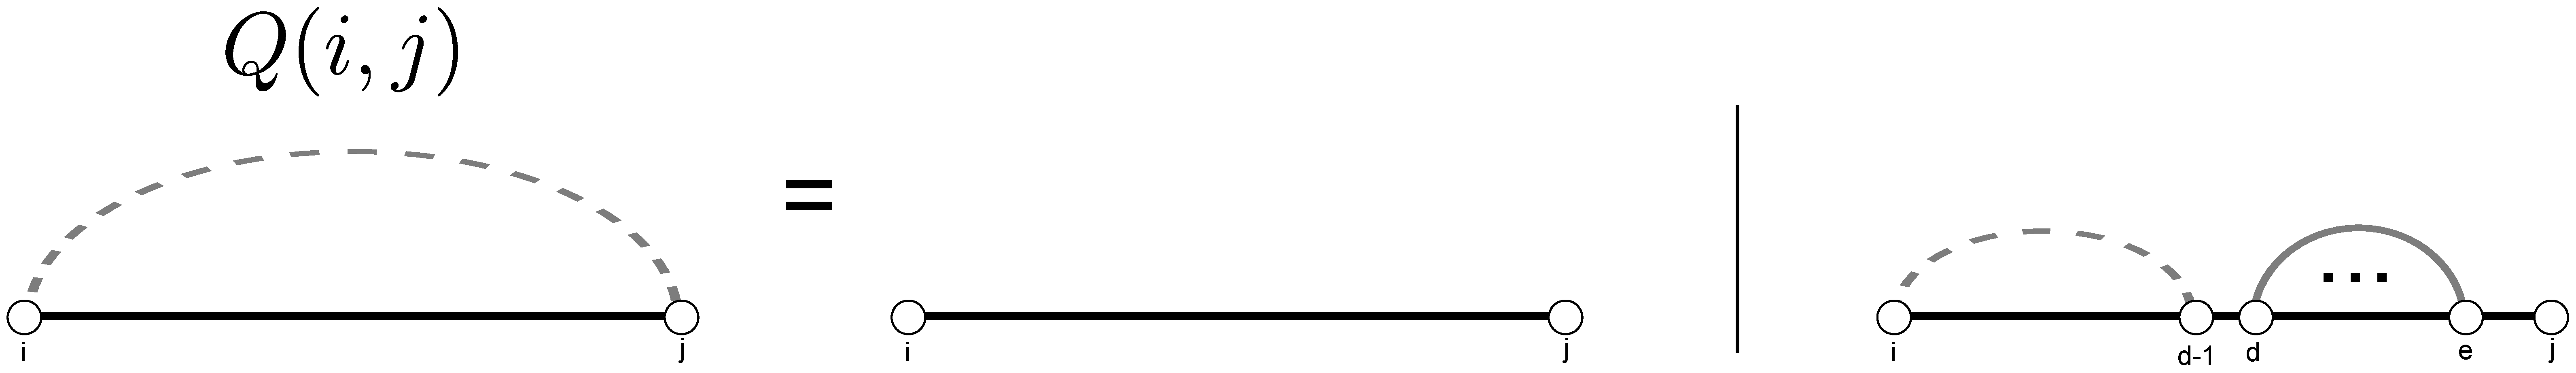
\includegraphics[width=\textwidth]{QijnewRecurrence.eps}
\caption{The recurrence relation for $Q(i,j)$. When we compute
  $Q(i,j)$ we only need to consider two cases, and add them together:
  either the strand will be empty of pairs, or there must be a
  rightmost pair followed plus whatever else is left, which can be
  represented as $Q(i, d-1)$. The partition function ``underneath''
  the rightmost pair is $Q^b(d, e)$, which is the partition function
  with $d$ and $e$ constrained to be paired. The mathematical formula
  corresponding to this diagram is in equation \ref{eq:Qij}.}
\label{fig:recurrenceRelationsQij}
\end{figure}
\begin{figure}[t]
\centering
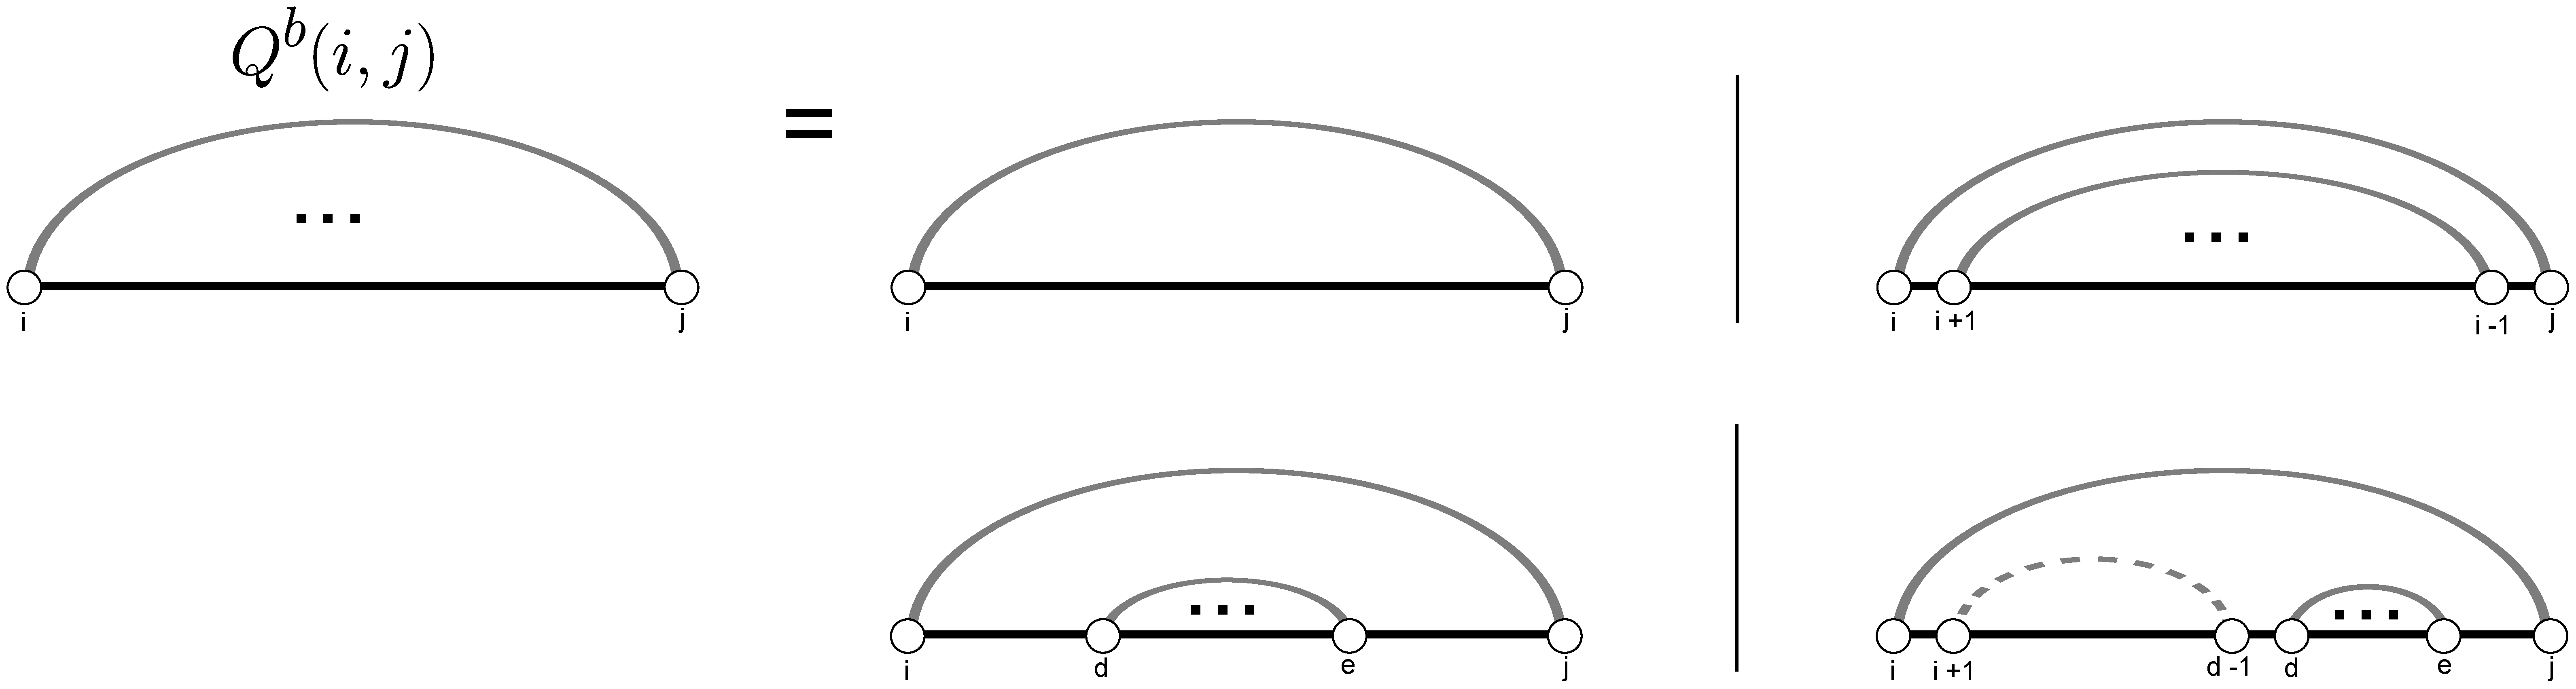
\includegraphics[width=\textwidth]{QbijRecurrence.eps}
\caption{The recurrence relation for $Q^b(i,j)$. We consider 4 cases,
  corresponding to each of the type of loop that could form under the
  $(i,j)$ pair, and add them together. The loop could form a hairpin,
  a stack loop, an internal loop, or a multi loop. The mathematical
  formula corresponding to this diagram is in equation \ref{eq:Qbij}.}
\label{fig:recurrenceRelationsQbij}
\end{figure}

Starting at the outermost layer, we compute $Q(i,j)$ by adding 2 cases
together, either the strand is empty on that interval or it has a
rightmost pair $(d,e)$ (see Figure
\ref{fig:recurrenceRelationsQij}). If it has a rightmost pair, the
partition function must be summed over every combination of structures
on the substrand $(i, d-1)$ as well as every structure that could form
underneath the pair $(d,e)$. Define:
\begin{equation}
Q^b(i, j) = \text{sum of boltzmann factors for every structure contained underneath pair } (i,j)
\end{equation}
Recalling Figure \ref{fig:attachedHairpin}, we can get every combination
of such states by multiplying $Q(i, d-1)$ by $Q^b(d,e)$ and an energy
penalty for leaving $(e+1, j)$ empty. Of course, it must be summed
over all possible indices $d$ and $e$:
\begin{equation} 
Q(i,j) = \overbrace{e^{-b(j-i+1)/RT}}^{\text{empty}} + \overbrace{\sum_{\substack{ d,e \\ i \leq d < e \leq j}}Q(i, d - 1) Q^b(d, e) e^{-b(j-e)/RT}}^{\text{rightmost pair}}. 
\label{eq:Qij}
\end{equation}

To compute $Q^b(i,j)$ we sum over the 4 cases of loops that could form
underneath the assumed pair $(i,j)$. This could mean a hairpin loop,
with energy function $E_h$, a stack loop, with $E_s$, an interior
loop, with $E_i$, or a multiloop with $a$, the multiloop penalty. For
each new pair created, we must multiply in $Q^b$ for that section as
well, and for every open region created, $Q$ (see Figure
\ref{fig:recurrenceRelationsQbij}).
\begin{equation}
\begin{split}
 Q^b(i, j) =& \overbrace{e^{-E_h(i,j)/RT}}^{\text{hairpin}} +
 \overbrace{e^{-E_s(i, j)/RT} Q^b(i+1, j-1)}^{\text{stack}} \\ 
& + \overbrace{\sum_{\substack{d,e \\ i < d< e< j}} E_i(i, d, e, j)Q^b(d,e)}^{\text{internal}} \\ 
& + \overbrace{e^{-a/RT} \sum_{\substack{d,e \\ i < d< e< j}} Q(i+1, d-1) Q^b(d,e) e^{-b(j-e-1)/RT}}^{\text{multiloop}}.
\end{split}
\label{eq:Qbij}
\end{equation}

Assuming that we've already computed and stored $Q(d,e)$ and
$Q^b(d,e)$ for all $(d,e)$ such that $ i \leq d < e \leq j$, each of
those functions is just a table lookup. Therefore the only
compute-bounding term is the sum over $d$ and $e$, which makes
computing $Q(i,j)$ an $O(n^2)$ computation, a big speed up over
$O(1.8^n)$. The same goes for $Q^b(i,j)$. One catch is that in order
to compute $Q(i,j)$ or $Q^b(i,j)$, you must compute all $O(n^2)$
$Q(d,e)$'s and $Q^b(d,e)$'s on the inside, so the entire algorithm is
actually $O(n^4)$ but there are known efficiency improvements that
bring it down to $O(n^3)$. This thesis presents improvements that
bring the algorithm down to $O(n^2)$, provided a good hueristic, in
the next section.

\section{Efficient Partition Function}

Let us assume that we have a huerstic of the form of a function 
\begin{equation}
K : \text{Base Index} \to \text{[Base Index]},
\end{equation}
that takes the index of a base as input and outputs a list of other
bases it can pair to, where the length of this list is always very
short and can be considered constant length in relation to the
sequence length $n$. This is not an unreasonable assumption in certain
cases. For example if we have already computed the partition function
of the strand but are now restricting certain bases from pairing, as
in Nestor PF clustering, we already know a lot about what pairs can
form. Another possibility could be restricting the base pairs based on
sequence alignment. We could also just restrict non-Watson-Crick pairs
to start. Importantly, we have seen empirically that the list of pairs
above a probability theshold for each base will be very short.

The problem terms of each computation are the sums over $d$ and
$e$. In order to get the algorithm down to $O(n^2)$ each $Q(i,j)$ and
$Q^b(i,j)$ must take constant time. Efficiency gains have already been
seen by McCaskill by limiting the internal loop length, introducing
the constraint that $(d-i) + (j-e) < L$ for some constant $L$. This
way, as $n$ computation is limited to $O(L^2)$ which is a
constant. That leaves only the multi-loop term to make a constant
time computation. Using the hueristic, this is possible. Let us define
a new function (and table) $Q^m(i, j)$ which is defined as (this time
explicitly summing $d$ and $e$):
\begin{equation}
Q^m(i, j) = \sum_{d = i}^{j}\sum_{e = d+1}^{j} Q(i, d-1)Q^b(d,e)e^{-b(j-e)/RT}.
\end{equation}
We can take the out all the terms which contain $e = j$ to split the
formula into two parts (note that I limited the first term's $d$ sum
to only go to $j-1$ because $d$ must always be less than $e$):
\begin{equation}
\begin{split}
Q^m(i, j) =& \sum_{d = i}^{j-1}\sum_{e = d+1}^{j-1} Q(i, d-1)Q^b(d,e)e^{-b(j-e)/RT} \\
&+ \sum_{d = i}^{j} Q(i, d-1)Q^b(d,j).
\end{split}
\end{equation}
The first term in this new equation is the same thing
$Q^m(i,j-1)e^{-b/RT}$. In the second term, it is always implied that
$d$ pairs with $j$, so we can substitute the summation index for our
hueristic for $j$, $K(j)$, without losing anything. Therefore, our
formula becomes:
\begin{equation}
Q^m(i, j) = Q^m(i, j -1) e^{-b/RT} + \sum_{k \in K(j)} Q(i, k - 1) Q^b(k, j).
\end{equation}
Now, we can examine the efficiency of computing $Q^m(i,j)$. The first
term is a constant factor and the second is a sum over only a constant
number of indices by our empirical assumptions about the
hueristic. Therefore the computation of $Q^m$ can be treated as a
constant time computation.

Now the computation for $Q(i,j)$ becomes:
\begin{equation}
Q(i,j) = e^{-b(j-i+1)/RT} + Q^m(i, j),
\end{equation} 
and for $Q^b(i,j)$:
\begin{equation}
\begin{split}
 Q^b(i, j) =& e^{-E_h(i,j)/RT}+
e^{-E_s(i, j)/RT} Q^b(i+1, j-1) \\ 
& + \sum_{\substack{d,e \\ i < d< e< j\\ (d-i) + (j-e) < L}} E_i(i, d, e, j)Q^b(d,e) \\ 
& + e^{-a/RT}Q^m(i+1, d-1) .
\end{split}
\end{equation}

So assisted by this hueristic we are able to reduce all table updates
to constant time computations. This means the algorithm is only
limited by the number of $(i,j)$'s which grows with $O(n^2)$. 

\section{Results}

Calculating the partition function is still difficult, but it can be
improved in the asymptotic case. The results show that the new
computation has a large constant factor in the beginning of the
algorithm. This could be related to the way the internal loop sum is
calculated, if $L=30$, the constant attached the the loop sum is
$L^2=900$. This constant term will only stop dominating as the number
of bases gets much larger than 900, as we can see by the plot. If we
reduce $L$, we should also see a reduction in  probability barrier, we
get further reductions in runtime.

\begin{figure}
\centering
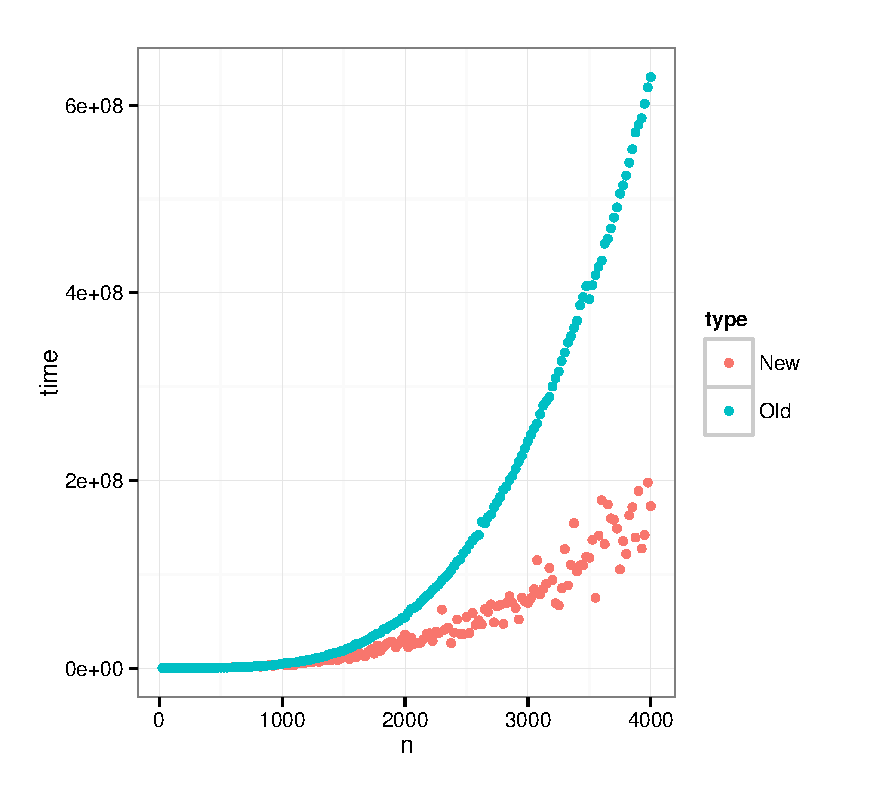
\includegraphics[width=\textwidth]{partitionTimePlot.eps} 
\caption{Computation time vs length for random sequences, the old
  $O(n^3)$ partition function run against the new $O(n^2)$ partition
  function. Not quite the results we were after, however, we can
  always set the max internal loop length $L$ to a lower value and
  increase the probability threshold $\theta$.}
\label{fig:pfResults}
\end{figure}

[TODO: include plot with different times for different probability
thresholds]

A large part of the verification of an improved algorithm is showing
that it produces acceptable results compared to the old algorithm, as
you can see in the plot, our algorithm gives the same results up to 1
part in 1 million [TODO: check this]. Increasing the probability
threshold changes the results by [TODO: find out].

[TODO: include plot of verification]

\section{Conclusion}

The partition function computation is hard and is a limiting factor in
RNA structure prediction. However, given a heuristic to predict the
base pairs, we can make the algorithm run much faster. These
improvements can be used in applications such as clustering based on
our nestedness measure, using the partition function. These
improvements also open up several possible branches for further
investigation. Can a heuristic be generated before the partition
function is computed, so that the pairs can be restricted and the
computation done in much faster time than the $O(n^3)$ algorithm?
Could this concept be applied to the pseudoknot algorithm to possibly
speedup the computation for that as well? Applications of this sort
could have tremendous impact on RNA secondary structure prediction,
opening up incredible avenues of potential.

